\documentclass[10pt,twocolumn,a4paper]{article}

\usepackage[utf8]{inputenc}
\usepackage[T1]{fontenc}
\usepackage[margin=1.6cm,columnsep=0.6cm]{geometry}
\usepackage{amsmath,amssymb}
\usepackage{graphicx}
\usepackage{booktabs}
\usepackage{eurosym}
\usepackage{xcolor}
\usepackage[hidelinks]{hyperref}
\usepackage{titlesec}
\usepackage{enumitem}

\graphicspath{{../results/figures/}}
\titlespacing*{\section}{0pt}{6pt}{3pt}
\titlespacing*{\subsection}{0pt}{4pt}{2pt}
\setlist{nosep,leftmargin=*}
\setlength{\parskip}{2pt}
\setlength{\abovecaptionskip}{3pt}
\setlength{\textfloatsep}{6pt}

% Texte à compléter quand les résultats du Q-learning seront disponibles
\newcommand{\todo}[1]{\textcolor{red}{[TODO: #1]}}

\title{\vspace{-1.2cm}\textbf{Plan or Learn? Dynamic Pricing of Airline Tickets under Model Error}}
\author{Imane Amraoui \and Dia Eddine Kadri\\
\small Reinforcement Learning course (J.~Martinet), Polytech SI5-IAID, 2026--2027\\
\small Code: \url{https://github.com/kadridiaa/airline-dynamic-pricing-RL}}
\date{\vspace{-0.8cm}}

\begin{document}
\maketitle

\section{Introduction}
An airline sells the seats of a flight over 30 days and sets a price every day.
If the demand model is known, Dynamic Programming (DP) computes the optimal pricing policy.
In practice the model is estimated, hence wrong.
Model-free temporal-difference learning (Q-learning) needs no model, only interaction, but needs many episodes.
\textbf{Research question:} from which level of model error does learning without a model (Q-learning) outperform planning with a wrong model (DP), for a given budget of episodes?

\section{Problem formulation}
\textbf{MDP.} The state is $s=(c,t)$ with $c\in\{0,\dots,10\}$ seats left and $t\in\{0,\dots,30\}$ days to departure.
The six actions are prices $p\in\{50,80,110,140,170,200\}$\,\euro.
Selling $k$ seats gives the reward $r=p\,k$ and the transition $(c,t)\to(c-k,\,t-1)$; the episode ends at departure ($t=0$) or when the plane is full ($c=0$).
We use $\gamma=1$ (finite horizon), which gives 341 states and 2\,046 state-action values.
Keeping $t$ in the state makes the process Markov: the optimal price depends on the time left.

\textbf{Demand model.} Two customer segments arrive as Poisson processes:
leisure customers ($\lambda_L=0.8$/day if $t>10$, $0.3$ otherwise) and business customers ($\lambda_B=0.1$, then $1.0$ in the last 10 days).
Willingness to pay (WTP) is exponential with mean $m_L=80$\,\euro{} and $m_B=180$\,\euro, so a customer buys with probability $e^{-p/m}$.
By Poisson thinning, daily demand is $D\sim\mathrm{Poisson}(\mu)$ with $\mu(t,p)=\lambda_L(t)e^{-p/m_L}+\lambda_B(t)e^{-p/m_B}$, and sales are $k=\min(D,c)$, hence $P(k=c)=P(D\ge c)$.

\textbf{Capacity.} With 20 seats, even at 50\,\euro{} only 19.3 customers buy on average: the plane is almost never full and a myopic policy (maximising today's revenue, i.e.\ $\gamma\approx 0$) loses only 0.1\,\%.
With $C=10$, ignoring the future costs 18.9\,\%, the load factor is 77\,\% and 23\,\% of flights sell out.
What matters is the demand/capacity ratio, not the absolute number of seats.

\section{Methods}
\textbf{DP.} The Bellman optimality equation reads
\begin{equation*}
V^*(c,t)=\max_a \sum_{k=0}^{c} P(k\mid c,t,a)\,\big[p_a k+\gamma V^*(c-k,\,t-1)\big],
\end{equation*}
with $V^*(c,0)=V^*(0,t)=0$.
Since $V^*(\cdot,t)$ only depends on $V^*(\cdot,t-1)$, a single backward sweep from $t=1$ to $t=30$ is exact (no iteration to convergence is needed, unlike value iteration in infinite horizon).

\textbf{Model error.} The DP receives a demand model in which both WTP means are multiplied by $(1+x)$, $x\in[-50\,\%,+50\,\%]$.
We perturb the WTP rather than the arrival rates because an error on $\lambda$ costs the DP at most 5\,\% of revenue.

\textbf{Q-learning and SARSA.} Tabular, $Q=0$ at start, $\varepsilon$-greedy exploration with $\varepsilon$ starting at 1 and decaying; off-policy update $Q(s,a)\leftarrow Q(s,a)+\alpha\,[r+\gamma\max_{a'}Q(s',a')-Q(s,a)]$, and the on-policy SARSA variant. They only interact with the simulator and never see the model.
\todo{final $\alpha$ and $\varepsilon$ schedule (issue \#14)}

\textbf{Baselines.} Best fixed price, and best linearly rising price schedule (21 start/end pairs).

\textbf{Evaluation.} Every policy is scored by the same function on the \emph{true} model: exact policy evaluation (finite-horizon iterative policy evaluation), cross-checked with 10\,000 simulated flights.
The metric is the percentage of the optimal revenue; learning methods use 10 seeds.
Consistency checks: the DP value lies in the 95\,\% confidence interval of its simulated revenue, and no wrong-model DP or baseline beats the true-model DP.

\section{Results}
\begin{table}[t]
\centering\small
\begin{tabular}{@{}lrrr@{}}
\toprule
Policy (true model) & Revenue & \% opt. & Load \\
\midrule
DP (optimum) & 1\,193.5\,\euro & 100.0 & 77\,\% \\
Rising price 140$\to$170\,\euro & 1\,166.1\,\euro & 97.7 & 74\,\% \\
Fixed price 170\,\euro & 1\,146.7\,\euro & 96.1 & 68\,\% \\
Q-learning & \todo{} & \todo{} & \todo{} \\
SARSA & \todo{} & \todo{} & \todo{} \\
\bottomrule
\end{tabular}
\caption{Expected revenue per flight ($C=10$, $T=30$).}
\label{tab:main}
\end{table}

\textbf{Optimal policy} (Fig.~\ref{fig:policy}). The price never increases with the number of seats left, jumps to 170\,\euro{} or more when business customers arrive ($t\le 10$), and, with many seats left, drops to 80\,\euro{} at $t=11$--$12$ to sell to the last leisure customers.
A simple rising schedule already reaches 97.7\,\% (Table~\ref{tab:main}): the value of planning over a well-tuned heuristic is small.

\begin{figure}[t]
\centering
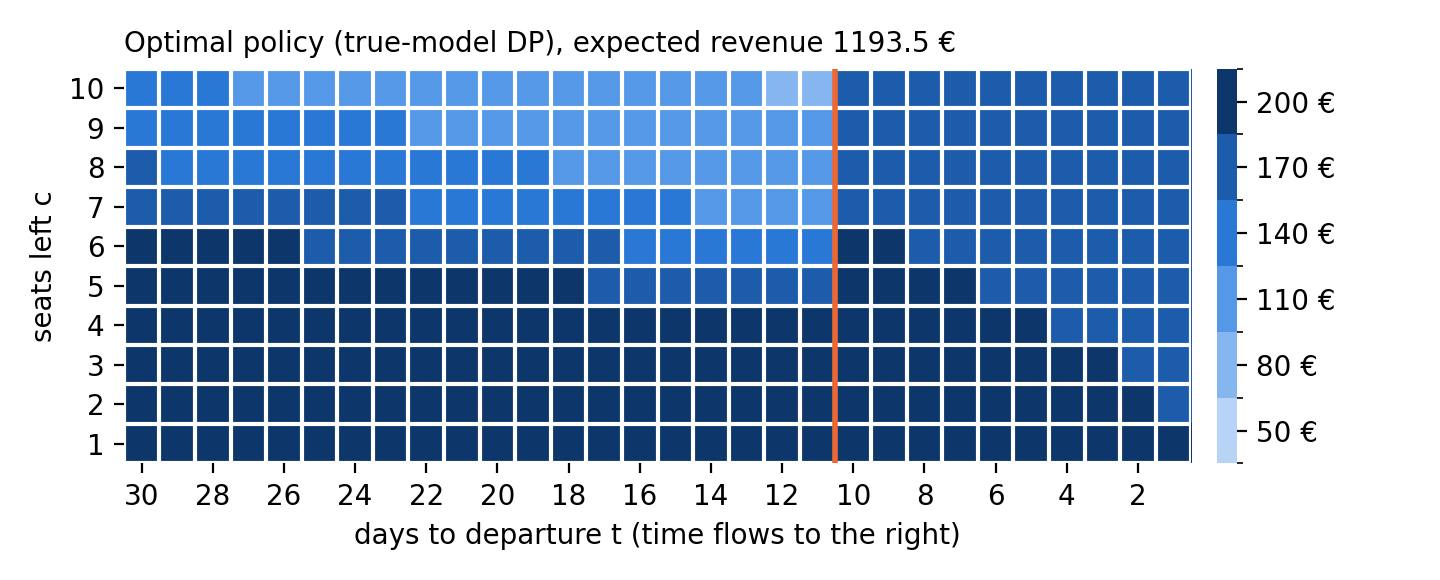
\includegraphics[width=\columnwidth]{policy_dp.png}
\caption{Optimal DP policy: price as a function of seats left and days to departure. Business customers arrive from $t=10$ (orange line).}
\label{fig:policy}
\end{figure}

\textbf{Planning with a wrong model} (E2, Fig.~\ref{fig:e2}). The DP stays above 97\,\% of the optimum for $|x|\le 20\,\%$.
Errors are asymmetric: underestimating the WTP ($x=-50\,\%$) yields 75.8\,\% because the plane sells out too cheaply (88\,\% of flights full), against 92.9\,\% at $x=+50\,\%$.
For the same wrong model, the DP always beats the rising-price heuristic tuned on that model.
\todo{Q-learning level for each budget of episodes, and tipping point (E2)}

\begin{figure}[t]
\centering
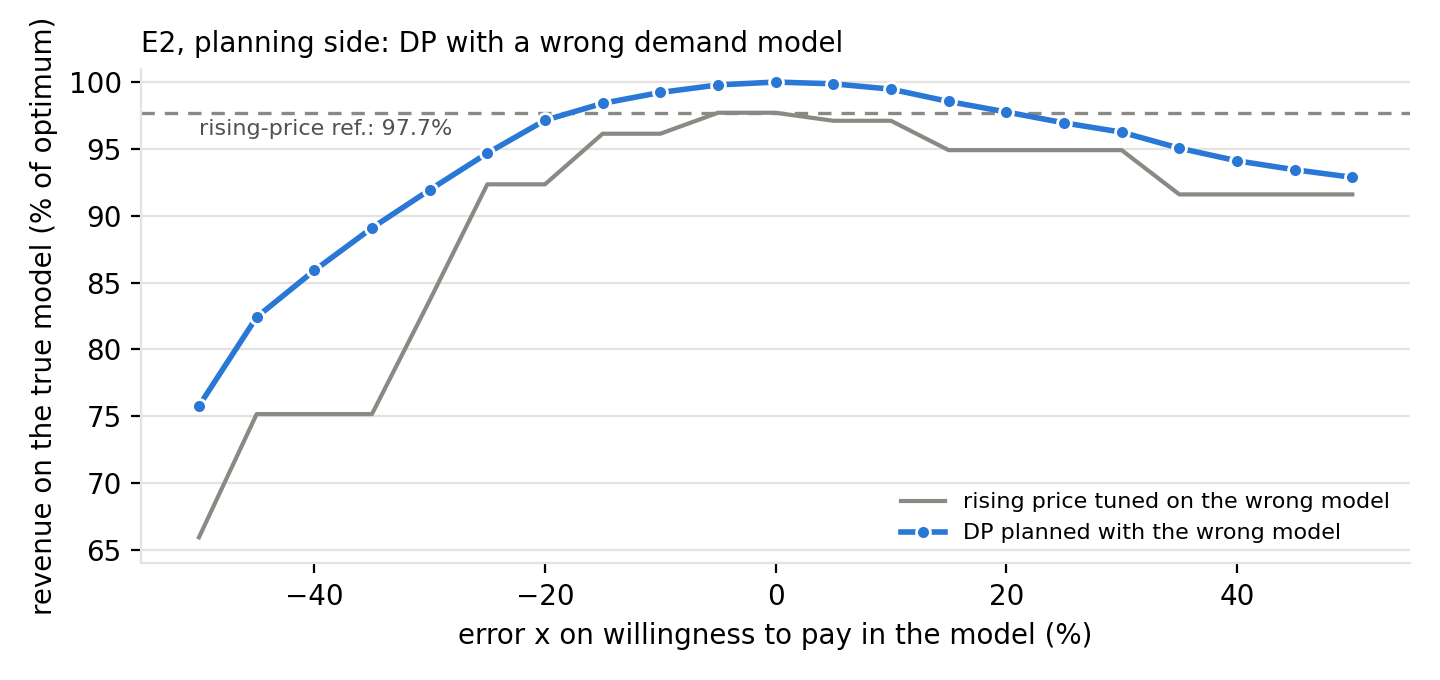
\includegraphics[width=\columnwidth]{e2_dp_side.png}
\caption{E2: revenue on the true model of the DP planned with a wrong WTP. \todo{add Q-learning levels per budget}}
\label{fig:e2}
\end{figure}

\todo{E1: episodes to reach 95\,\% of the optimum. E3: Q-learning vs DP policies. E4: effect of $\gamma\in\{1,0.9,0.5\}$.}

\section{Discussion and conclusion}
\todo{answer to the research question: tipping point between planning and learning.}
The advantage of planning over a simple heuristic is small (2.3\,\%), so a moderate model error is enough to lose it; and the direction of the error matters more than its size.
\textbf{Limitations:} synthetic demand, a single perturbed parameter, tabular methods.
\textbf{Perspective:} realistic aircraft (150+ seats) make tabular methods impractical; value function approximation would be needed.

\begin{thebibliography}{9}\small
\setlength{\itemsep}{0pt}
\bibitem{sutton} R.~S.~Sutton and A.~G.~Barto. \emph{Reinforcement Learning: An Introduction}, 2nd ed., MIT Press, 2018.
\bibitem{gallego} G.~Gallego and G.~van Ryzin. Optimal dynamic pricing of inventories with stochastic demand over finite horizons. \emph{Management Science}, 40(8):999--1020, 1994.
\end{thebibliography}

\end{document}
